\chapter{Execução da Pesquisa}


\section{Ferramentas Aplicadas}

O código será versionado no
Github\footnote{\url{https://github.com/diegofreitas/platform_packages_apps_contacts}}
onde será feito o gerenciamento das versões de cada iteração.
As ferramentas utilizadas para a refatoração serão a IDE Eclipse(Juno) com
plugin ADT v21 para facilitar a edição do código e ferramentas de construção
do projeto existentes no próprio repositório do android, tendo em vista que todo
o processo de compilação e empacotamento não visa ser usado em uma IDE.
Para realizar a coleta das métricas é necessário que a ferramenta analise código
java e contemple todas as métricas descritas na seção \ref{sec:metrics}. O
programa Chidamber and Kemerer Java
Metrics(CKJM)\footnote{\url{https://github.com/dspinellis/ckjm}} atende esses
critérios, além de ser um projeto de código aberto. O CKJM é uma aplicação java
sem interface gráfica, executado por linha de comando. Ele analisa o código java
compilado, conhecido como byte codes contido em arquivos com extensão .class. Um
exemplo de uso do CKJM é mostrado a seguir:

\begin{figure}[!h]
	\centering
	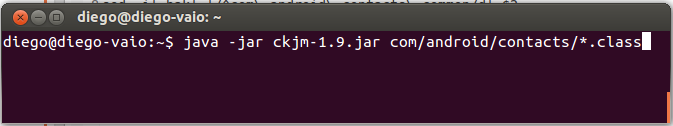
\includegraphics[scale=0.5]{img/ckjm_run.png}
	\caption{Exemplo de execução do CKJM} 
	\label{fig:ckjm_run}
\end{figure}


Os resultados são escritos na saída padrão do sistema, neste caso, no terminal
de execução, mostrando uma lista com os nomes completos das classes
analisadas, seguidas dos respectivos valores das métricas na seguinte
ordem: WMC, DIT, NOC, CBO, RFC, LCOM, Ce, and NPM sendo que as métricas Ce e
NPM são desconsideradas para esta pesquisa. a figura~\ref{fig:ckjm_result}
ilustra o resultado de uma coleta.


\begin{figure}[!h]
	\centering
	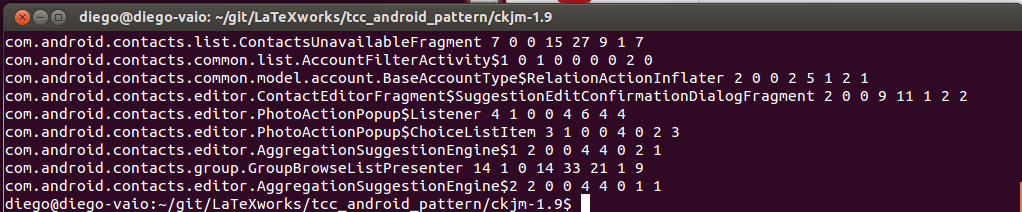
\includegraphics[scale=0.45]{img/ckjm_result.png}
	\caption{Exemplo de resultado da análise do CKJM} 
	\label{fig:ckjm_result}
\end{figure}


\section{Análise do objeto de estudo}

O aplicativo a ser refatorado tem funcionalidades para gerenciamento de
contatos e é composto 153 classes organizadas em 13 pacotes. O padrão
de projeto MVP será aplicado em uma parte do aplicativo. Será refatorado o
pacote referente ao gerenciamento de grupos de contatos presente no pacote
\textbf{com.android.contacts.group}. A figura \ref{fig:pacotes_contacts}
mostra os pacotes que compõem o aplicativo. O pacote a ser refatorado está
destacado em azul.

\begin{figure}[!h]
	\centering
	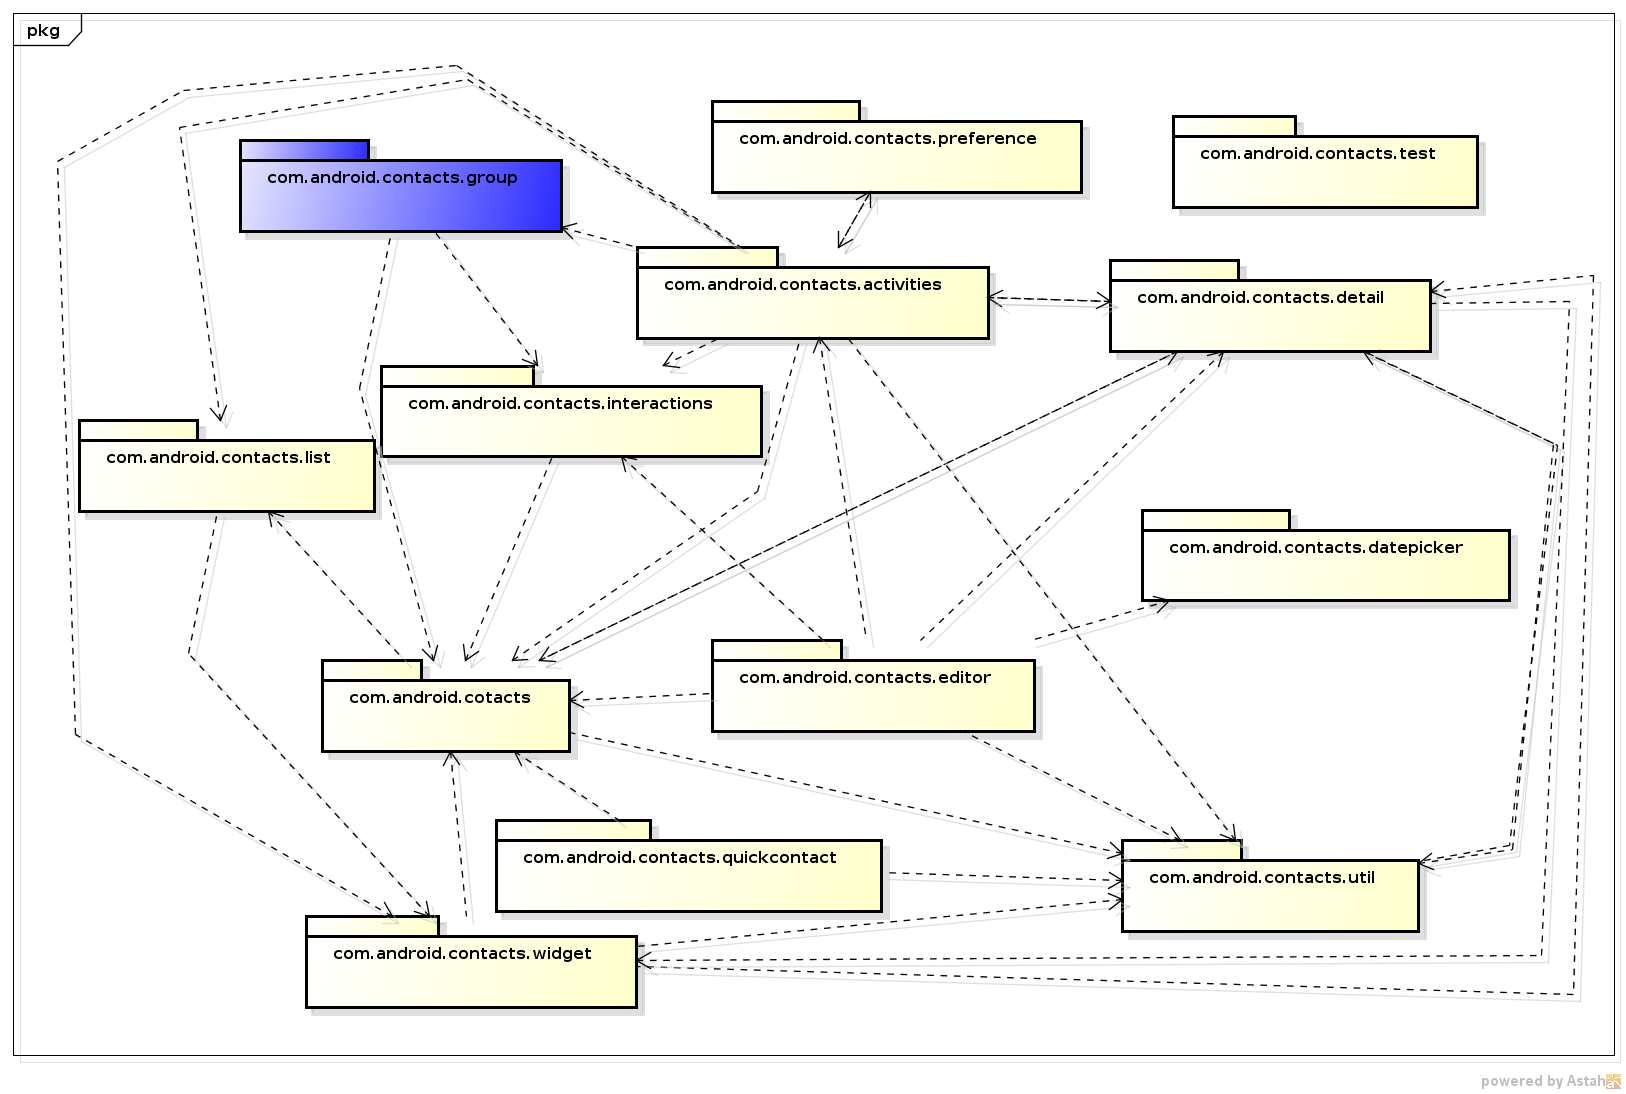
\includegraphics[scale=0.40,angle=90]{img/pacotes_contacts.png}
	\caption{Diagrama de pacotes do aplicativo de contatos} 
	\label{fig:pacotes_contacts}
\end{figure}


A cada iteração será selecionada uma tela do aplicativo para a aplicação do
padrão MVP. Cada tela é implementada por uma classe e suas interfaces
são ilustradas nas figuras \ref{fig:contacts_groups},
\ref{fig:contacts_groups_view} e \ref{fig:groups_edit}. 

\begin{figure}[!ht]
	\centering
	\begin{minipage}[b]{0.45\linewidth}
		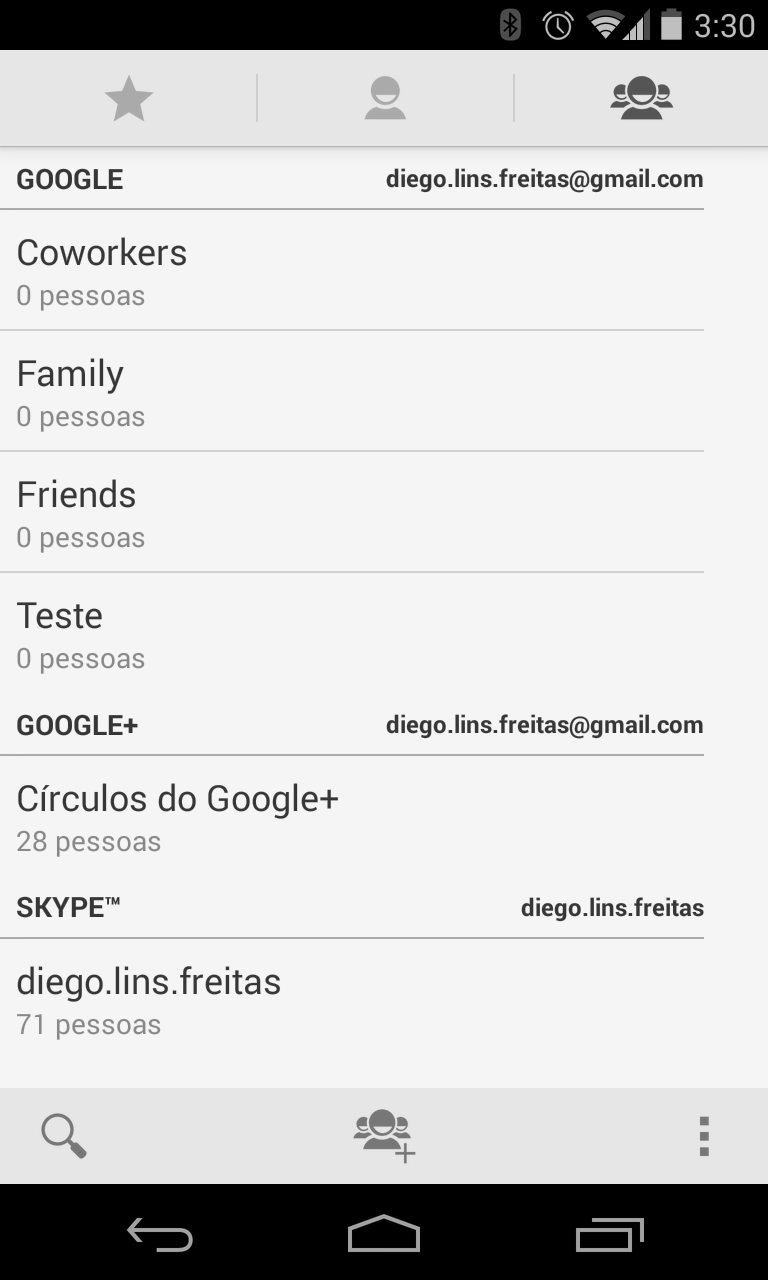
\includegraphics[scale=0.2]{img/contacts_groups.png}
		\caption{Tela de lista de grupos} 
		\label{fig:contacts_groups}
	\end{minipage}
\quad
	\begin{minipage}[b]{0.45\linewidth}
		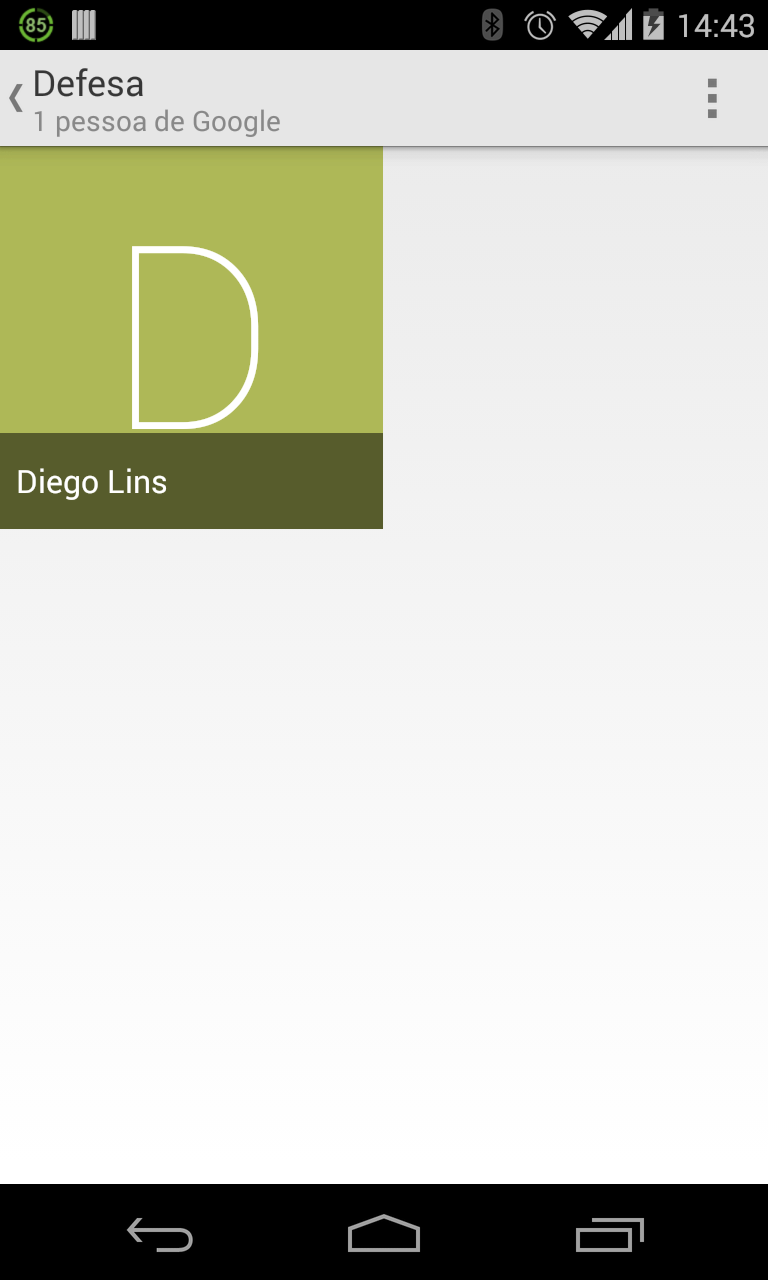
\includegraphics[scale=0.2]{img/contacts_group_view.png}
		\caption{Tela de visualização de um grupo} 
		\label{fig:contacts_groups_view}
	\end{minipage}
\quad
	\begin{minipage}[b]{0.45\linewidth}
		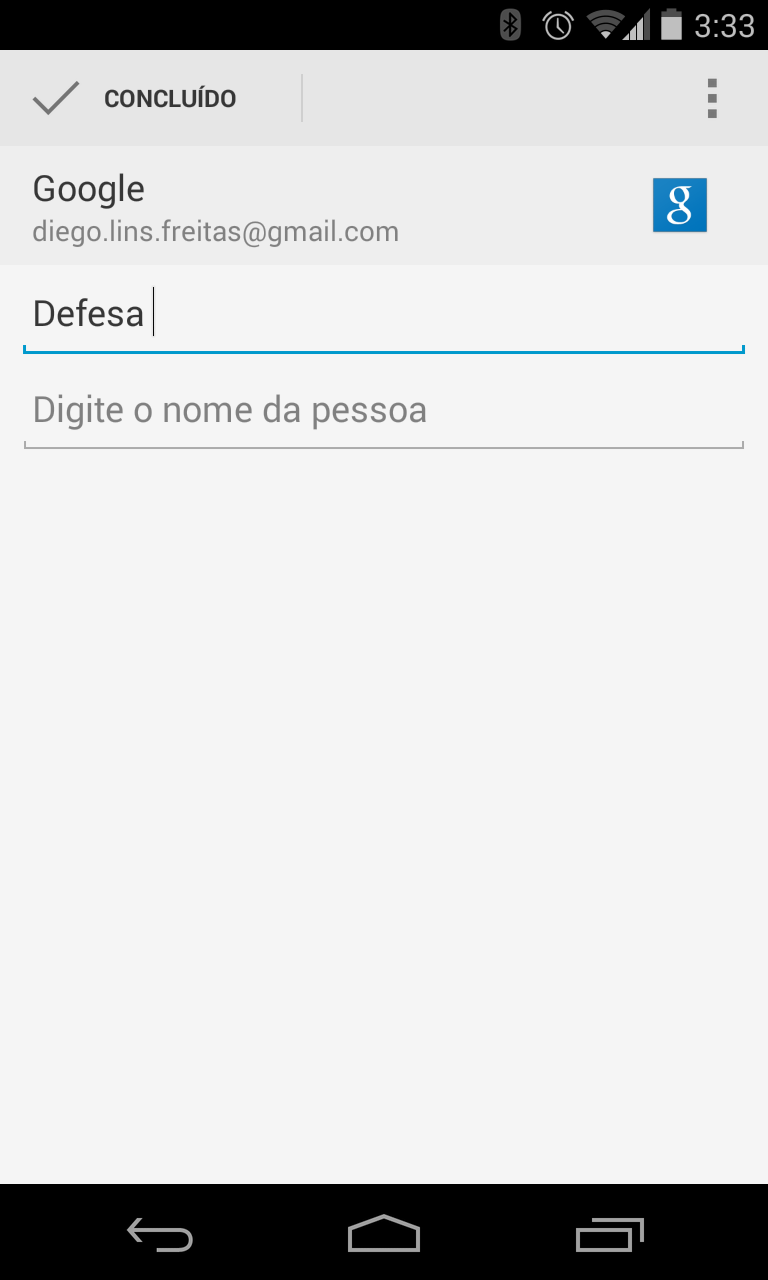
\includegraphics[scale=0.2]{img/contacts_edit.png}
		\caption{Tela de edição e criação de grupos} 
		\label{fig:groups_edit}
	\end{minipage}
\end{figure}


As classes a serem refatoradas são:
\begin{description}
\item[GroupDetailFragment.java] Exibe os dados de um grupo de contatos.
\item[GroupBrowseListFragment.java] Fornece uma lista de grupos.
\item[GroupEditorFragment.java] Disponibiliza um formulário para edição dos
dados de um grupo.
\end{description}

Essas classes estão presentes no pacote \textbf{com.android.contacts.group} como
mostra a figura \ref{fig:classes_group_baseline}.

\begin{figure}[!h]
	\centering
	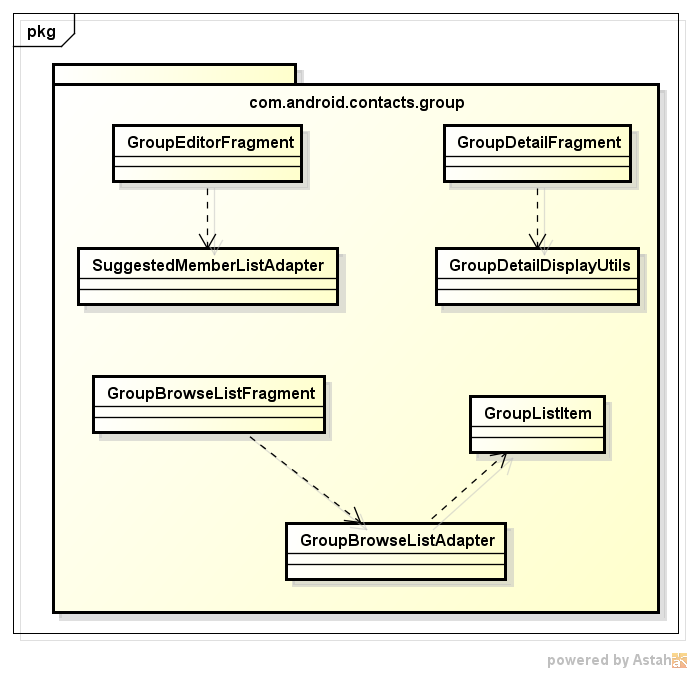
\includegraphics[scale=0.53]{img/classes_group_baseline.png}
	\caption{Diagrama de pacotes do aplicativo de contatos} 
	\label{fig:classes_group_baseline}
\end{figure}

Estas interfaces com o usuário são usadas dentro de Activities que controlam uma
parte do fluxo de interação e se comportam de forma diferente conforme o tipo de dispositivo
móvel utilizado (tablet ou smartphone). Devido a essa complexidade, não será
feita nenhuma alteração na interface pública dos componentes refatorados, evitando efeitos colaterais em
outras partes do aplicativo. Os componentes elencados contêm código não somente
relacionado com a lógica de apresentação como também interagem diretamente com classes destinadas ao acesso
de dados e serviços existentes nas dependências do projeto, por exemplo,
gerenciamento de contas do usuário.  Cada iteração consistirá na refatoração de
cada um dos componentes descritos. O marco de referência de dados das métricas presentes na tabela \ref{tab:dados_baseline} será feita a partir da
versão \verb|4.4.2_r1| do aplicativo.

\begin{table}[!h]
	\centering
	    \caption{Métricas CK da versão de referência}
	
    \begin{tabular}{ | l | l | }
    \hline
    Métrica &	Média \\ \hline
    WMC  	&	8.5161290323   	\\ \hline
    DIT	 	&	0.7741935484	\\ \hline
	NOC  	& 	0				\\ \hline
	CBO	  	& 	10.1612903226	\\ \hline
	RFC	 	& 	23.7419354839	\\ \hline
	LCOM 	& 	57.4838709677	\\ \hline
    \end{tabular}
    \label{tab:dados_baseline}
\end{table}


\section{Arquitetura Proposta}

Será aplicado nos experimentos a variação do padrão MVP chamada Passive View,
pois dessa forma, o Model não precisa publicar alterações de seu estado para a
view, Logo, evita-se alterações no código referente às classes que fazem
parte da camada de Model do aplicativo de contatos. A organização do código
fonte no repositório dificulta a implementação, isto porque esses componentes estão
localizados fora do projeto afetado e são compartilhados.

As classes que extendem Fragment terão a responsabilidade da View, pois é neste
componente que a interface com o usuário é construída. A classe Activity fornece
vários métodos para recuperação de recursos de imagens, textos, inicialização de
serviços, entre outros. Isso ocorre porque a classe Activity é uma subclasse de Context, herdando diversos métodos não relacionados ao gerenciamento da interface.

Segundo \citeonline{Reenskaug:1979} ``\ldots Os papéis da View e do
Controller podem ser exercidos pelo mesmo objeto quando eles estão muito
acoplados. Exemplo: Um Menu.''(tradução livre). Porém, isso requer um boa
análise do problema em questão para decidir o nível de granularidade que esses componentes podem ter.
Portanto, é recomendável manter sempre essa separação para manter uma boa coesão
nas classes. O Presenter será uma classe auxiliar à View e pode ser implementada
como uma classe java simples. 



\section{Resultados dos Experimentos}

Esta seção tem como objetivo mostrar os resultados obtidos com o processo de
refatoração aplicando o parão MVP. Cada métrica é apresentada com seus dados
para cada iteração mostrando os efeitos desses valores na qualidade.

\subsection{WMC}

%1o) qual o cenario ideal para metrica;
A métrica WMC é usada para medir o tempo e esforço necessário para desenvolver e
manter uma classe. Levando em consideração o método como uma unidade de
complexidade, quanto menos métodos um classe tiver menos complexa ela será,
portanto, é recomendado que esta métrica tenha valores baixos.
Entretanto, uma classe terá a quantidade de métodos necessária para exercer seu
papel no sistema. É inviável desenvolver um sistema cujas todas as classes
tenham um único método com a implementação de todas as funcões de uma
classe. Portanto, não existe um valor ideal para a métrica WMC. Essa métrica
deve ser analisada levando em consideração o contexto da classe de interesse além da
complexidade expressa pela quantidade de métodos. 

A possibilidade de reuso de uma classe reduz, pois a grande quantidade de
métodos indica que ela tem funções muito específicas\cite{cksuite}. Neste caso o
WMC é um indicador de que é necessário fazer um refatoração para extrair funções comuns a outras partes do
aplicativo, além do pacote de Groups, como por exemplo funções para exibição de
dados em uma lista, validação de dados em componentes de texto, entre outros. O
escopo de atuação do padrão MVP é mais amplo, abrangendo o caso de uso realizado pela
interface refatorada. Logo, o MVP não tem impacto na reusabilidade.

Os efeitos colaterais em uma classe filha é maior quando é feito alguma
alteração na classe pai que tenha o número de métodos muito alto\cite{cksuite}.
Isso dificulta a manutenabilidade e o esforço de testes. Porém, As classes
refatoradas tem uma função muito específica dentro da aplicação e não são
extendidas por outras classes. O MVP está relacionado com a separação de
responsabilidades e sua aplicação não interferiu na hierarquia de classes que
foram refatoradas.
A tabela \ref{tab:wmc} e a figura \ref{fig:wmc} mostram os valores dessa
métrica no projeto.


\begin{table}[!h]
	\centering
	\caption{Dados métrica WMC}
    \begin{tabular}{ | l | l | }
    \hline
    Iteração & Média 			\\ \hline
    Baseline & 8.5161290323   	\\ \hline
    Iteração 1 & 8.875			\\ \hline
	Iteração 2 & 9				\\ \hline
	Iteração 3 & 8.9393939394	\\ \hline
    \end{tabular}
    
    \label{tab:wmc}
\end{table}

\begin{figure}[!h]
	\centering
	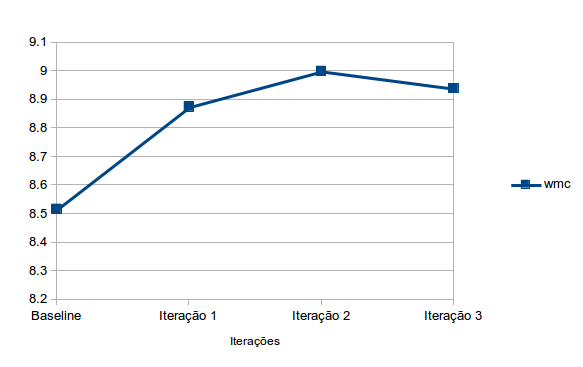
\includegraphics{img/wmc.png}
	\caption{Gráfico da métrica WMC/Fonte: Próprio autor} 
	\label{fig:wmc}
\end{figure}

%3o) justificar o q causou tal comportamento.

De acordo com o que foi exposto, o MVP não deveria afetar a métrica WMC. Porém,
houve um aumento nos valores dessa métrica . Isso é consequência da divisão de
responsabilidades entre a View e o Presenter. Antes da refatoração, os métodos
das classes de View implementavam o acesso a dados, controle dos componentes
visuais e regras específicas das operações executadas na tela, como por exemplo,
a atualização de um componente visual quando nenhum dado está disponível para
exibição. Os métodos da classe de View, afetados pela refatoração, foram
dividídos em no mínimo dois métodos. Sendo que, o método que permanece na View
manipula os componentes visuais, enquanto o novo método criado no Presenter faz
o acesso à camada de Model e implementa as regras de negócio da operação em
resposta à interação do usuário na View. Como consequência a quantidade de
métodos aumenta, porém, os métodos tornam-se mais simples pois implementam
funcões específicas. 

Levando isso em consideração, apesar dos valores de WMC
terem aumentado, a complexidade diminuiu, pois os métodos estão mais concisos.
No contexto dessa refatoração, a métrica WMC não pode ser considerada um
indicador determinante para a avaliação da qualidade do objeto de estudo.


\subsection{DIT}

A métrica DIT está relacionada complexidade e reusabilidade. Quanto mais
abaixo na hierarquia de herança a classe estiver, menos previsível será seu
comportamento devido a quantidade de métodos que serão herdados das classes
acima nessa hierarquia. Entretanto, a métrica também indica um potencial reuso
de código por meio da herança de métodos, isso torna os parâmetros de avaliação
da métrica dependentes do contexto a ser analisado. O aumento demonstrado na DIT
se deve ao fato que o CKJM considera a implementação de interface como herança.
A interface define somente o contrato que a classe deve implementar. Sendo uma
interface, não há nenhuma implementação que possa interferir no comportamento
da classe, portanto essa alteração na métrica DIT não deve ser considerada. O
aumento no valor da métrica é mostrado na tabela~\ref{tab:dit} e
figura~\ref{fig:dit}

\begin{table}[!h]
	\centering
	    \caption{Dados métrica DIT}
    \begin{tabular}{ | l | l | }
    \hline
    Iteração & Média 			\\ \hline
    Baseline & 0.7741935484  	\\ \hline
    Iteração 1 & 0.78125		\\ \hline
	Iteração 2 & 0.78125			\\ \hline
	Iteração 3 & 0.7878787879	\\ \hline
    \end{tabular}
    \label{tab:dit}
\end{table}

\begin{figure}[!h]
	\centering
	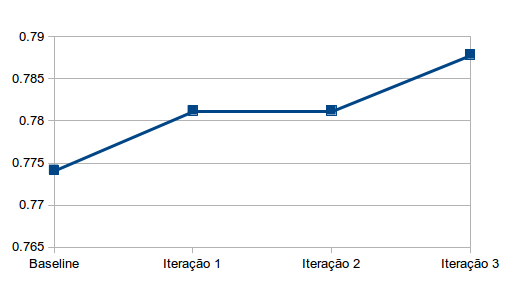
\includegraphics{img/dit.png}
	\caption{Valores de DIT/Fonte: Próprio autor}
	\label{fig:dit}
\end{figure}

\vspace{\onelineskip}
\vspace{\onelineskip}
\vspace{\onelineskip}
\subsection{NOC}

Altos valores para a métrica NOC são indicativos de que existe maior reuso de
código. Assim como DIT, a métrica NOC é um indicador da influência da classe
no comportamento das classes filhas o que aumenta o esforço de testes. Quando os
valores desta métrica estão aberrantes em relação às outras classes, há grande
chance de que a abstração está sendo usada de forma incorreta. Dado esses cenários, está é um métrica cujos
seus valores devem ser analisados caso a caso.

Durante o processo de refatoração não foi aplicada herança em nenhuma das
classes afetadas, portanto, essa métrica permaneceu intacta durante as iterações
como pode ser observado na tabela \ref{tab:noc}. %e figura~\ref{fig:noc}

\begin{table}[!h]
	\centering
	    \caption{Dados métrica NOC}
    \begin{tabular}{ | l | l | }
    \hline
    Iteração & Média 			\\ \hline
    Baseline & 0  	\\ \hline
    Iteração 1 & 0			\\ \hline
	Iteração 2 & 0				\\ \hline
	Iteração 3 & 0	\\ \hline
    \end{tabular}
    \label{tab:noc}
\end{table}

%\begin{figure}[h]
%	\centering
%	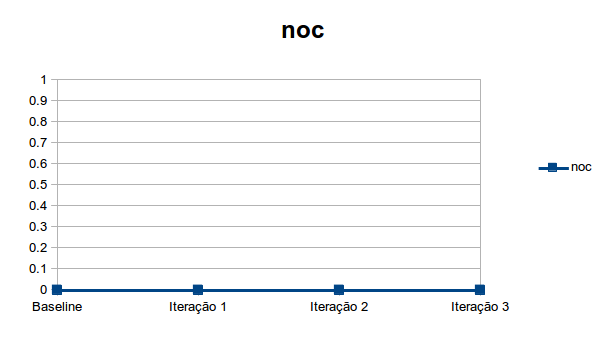
\includegraphics{img/noc.png}
%	\caption{Valores de NOC/Fonte: Próprio autor}
%	\label{fig:noc}
%\end{figure}

\subsection{CBO}

Valores baixos de CBO são indicativos de boa modularidade e encapsulamento que
se reflete na independência da classe, o que a torna mais fácil de reutilizar,
manter e testar.
Na primeira iteração foi aplicado o padrão em um componente mais simples e foi
possível remover qualquer dependência que não fosse relacionada a interface,
diminuinido significativamente o valor da métrica. Nas iterações seguintes foram
refatoradas interfaces mais complexas onde é mais difícil desacoplar as
dependências. Algumas depedências não relacionadas a camada de apresentação
permaneceram na View, dessa forma, tanto a View como o Presenter tem referências
para essas dependências aumentando o valor da métrica. Além disso, existe o
acréscimo de duas dependências entre a View e o Presenter. A variação da métrica
é exposta na tabela \ref{tab:cbo} e na figura~\ref{fig:cbo}

\begin{table}[!h]
	\centering
	    \caption{Dados métrica CBO}
	
    \begin{tabular}{ | l | l | }
    \hline
    Iteração & Média 			\\ \hline
    Baseline & 10.1612903226   	\\ \hline
    Iteração 1 & 10.03125		\\ \hline
	Iteração 2 & 10.09375		\\ \hline
	Iteração 3 & 10.1515151515	\\ \hline
    \end{tabular}
    \label{tab:cbo}
\end{table}

\begin{figure}[!h]
	\centering
	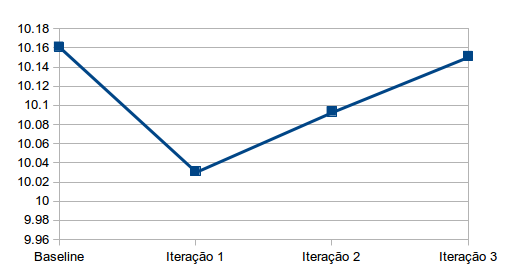
\includegraphics{img/cbo.png}
	\caption{Valores de CBO/Fonte: Próprio autor}
	\label{fig:cbo}
\end{figure}


\subsection{RFC}

Altos valores para a métrica RFC indica que uma quantidade grande de métodos são
chamados a partir de uma classe tornando-a mais complexa de testar e fazer
manutenção. Logo, esta métrica deve deve diminuir para expressar maior
qualidade no código. A métrica RFC tende a aumentar a cada iteração, o que
sugere um aumento da complexidade do código conforme é apresentado na tabela \ref{tab:rfc} e Figura
\ref{fig:rfc}.

\begin{table}[!h]
	\centering
	    \caption{Dados métrica RFC}
    \begin{tabular}{ | l | l | }
    \hline
    Iteração & Média 			\\ \hline
    Baseline & 23.7419354839   	\\ \hline
    Iteração 1 & 24.21875		\\ \hline
	Iteração 2 & 24.71875		\\ \hline
	Iteração 3 & 24.9090909091	\\ \hline
    \end{tabular}
    \label{tab:rfc}
\end{table}

\begin{figure}[!h]
	\centering
	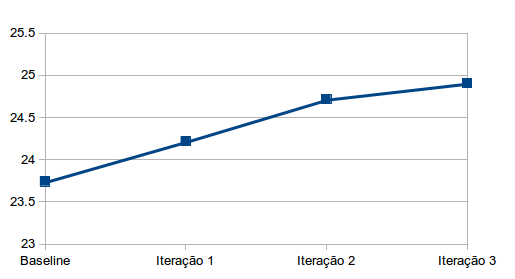
\includegraphics{img/rfc.png}
	\caption{Valores de RFC/Fonte: Próprio autor}
	\label{fig:rfc}
\end{figure}

A justificativa para o aumento da métrica WMC também se aplica neste caso.
Após cada iteração de refatoração, as Views passaram a delegar
responsabilidades para o Presenter por meio de chamada de métodos, além disso, o Presenter interage com a
View da mesma forma para atualizá-la. Portanto, a quantidade de chamada de
métodos aumentaram e isso se refletiu na métrica RFC.

\subsection{LCOM}

Segundo \citeonline{cksuite} ``Um valor alto de LCOM indica uma disparidade na
funcionalidade provida pela classe.". Analisando a relação entre os métodos da
classe e seus atributos é possível dizer se a classe tem muitas
responsabilidades e é necessário dividi-la em duas ou mais classes. Esta métrica
ajuda a identificar má qualidade na estrutura do código quando os valores são
altos, apontando aumento da complexidade e pouco encapsulamento. A tabela
\ref{tab:lcom} e a figura \ref{fig:lcom} mostram uma queda siginificativa na
métrica LCOM. Isto indica que a coesão do código melhorou após cada iteração.

\begin{table}[!h]
	\centering
	    \caption{Dados métrica LCOM}
    \begin{tabular}{ | l | l | }
    \hline
    Iteração & Média 			\\ \hline
    Baseline & 57.4838709677   	\\ \hline
    Iteração 1 & 56.875			\\ \hline
	Iteração 2 & 53.1875		\\ \hline
	Iteração 3 & 48.4242424242	\\ \hline
    \end{tabular}
    \label{tab:lcom}
\end{table}

\begin{figure}[!ht]
	\centering
	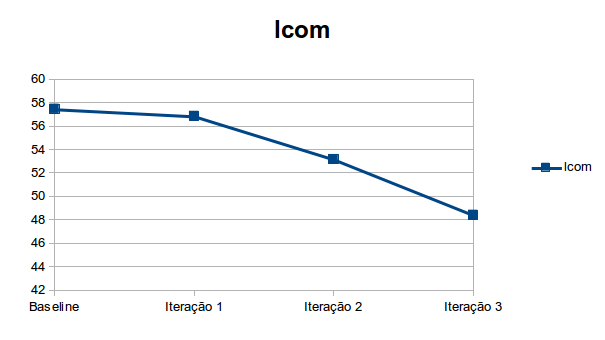
\includegraphics{img/lcom.png}
	\caption{Valores de lcom/Fonte: Próprio autor}
	\label{fig:lcom}
\end{figure}
